\chapter{Design Patterns} 

\label{appendix_b}

Extract from the Design Patterns: Elements of Reusable Object-Oriented Software\cite{design_patterns}.

\section{Singleton}

\subsection*{Intent}

Ensure a class only has one instance, and provide a global point of access to it.

\subsection*{Motivation}

It's important for some classes to have exactly one instance. Although there can be many printers in a system, there should be only one printer spooler. There should be only one file system and one window manager. A digital filter will have one A/D converter. An accounting system will be dedicated to serving one company.
\\\\
How do we ensure that a class has only one instance and that the instance is easily accessible? A global variable makes an object accessible, but it doesn't keep you from instantiating multiple objects.
\\\\
A better solution is to make the class itself responsible for keeping track of its sole instance. The class can ensure that no other instance can be created (by intercepting requests to create new objects), and it can provide a way to access the instance. This is the Singleton pattern.

\subsection*{Applicability}

Use the Singleton pattern when

\begin{itemize}
    \item there must be exactly one instance of a class, and it must be accessible to clients from a well-known access point.
    \item when the sole instance should be extensible by subclassing, and clients should be able to use an extended instance without modifying their code.
\end{itemize}

\subsection*{Structure}

\begin{figure}[H]
\centering
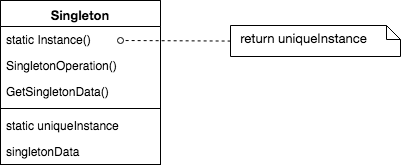
\includegraphics[scale=0.6]{diagrams/singleton.png}
\end{figure}

\subsection*{Participants}

\begin{itemize}
    \item Singleton
    \begin{itemize}
        \item defines an Instance operation that lets clients access its unique instance. Instance is a class operation (that is, a class method in Smalltalk and a static member function in C++).
        \item may be responsible for creating its own unique instance.
    \end{itemize}
\end{itemize}

\subsection*{Collaborations}

\begin{itemize}
    \item Clients access a Singleton instance solely through Singleton's Instance operation.
\end{itemize}

\subsection*{Consequences}

The Singleton pattern has several benefits:

\begin{enumerate}
    \item Controlled access to sole instance. Because the Singleton class encapsulates its sole instance, it can have strict control over how and when clients access it.
    \item Reduced name space. The Singleton pattern is an improvement over global variables. It avoids polluting the name space with global variables that store sole instances.
    \item Permits refinement of operations and representation. The Singleton class may be subclassed, and it's easy to configure an application with an instance of this extended class. You can configure the application with an instance of the class you need at run-time.
    \item Permits a variable number of instances. The pattern makes it easy to change your mind and allow more than one instance of the Singleton class. Moreover, you can use the same approach to control the number of instances that the application uses. Only the operation that grants access to the Singleton instance needs to change.
    \item More flexible than class operations. Another way to package a singleton's functionality is to use class operations (that is, static member functions in C++ or class methods in Smalltalk). But both of these language techniques make it hard to change a design to allow more than one instance of a class. Moreover, static member functions in C++ are never virtual, so subclasses can't override them polymorphically.
\end{enumerate}

\section{Adapter}

Also known as Wrapper.

\subsection*{Intent}

Convert the interface of a class into another interface clients expect. Adapter lets classes work together that couldn't otherwise because of incompatible interfaces.

\subsection*{Motivation}

Sometimes a toolkit class that's designed for reuse isn't reusable only because its interface doesn't match the domain-specific interface an application requires.
\\\\
Consider for example a drawing editor that lets users draw and arrange graphical elements (lines, polygons, text, etc.) into pictures and diagrams. The drawing editor's key abstraction is the graphical object, which has an editable shape and can draw itself. The interface for graphical objects is defined by an abstract class called Shape. The editor defines a subclass of Shape for each kind of graphical object: a LineShape class for lines, a PolygonShape class for polygons, and so forth.
\\\\
Classes for elementary geometric shapes like LineShape and PolygonShape are rather easy to implement, because their drawing and editing capabilities are inherently limited. But a TextShape subclass that can display and edit text is considerably more difficult to implement, since even basic text editing involves complicated screen update and buffer management. Meanwhile, an off-the-shelf user interface toolkit might already provide a sophisticated TextView class for displaying and editing text. Ideally we'd like to reuse TextView to implement TextShape, but the toolkit wasn't designed with Shape classes in mind. So we can't use TextView and Shape objects interchangeably.
\\\\
How can existing and unrelated classes like TextView work in an application that expects classes with a different and incompatible interface? We could change the TextView class so that it conforms to the Shape interface, but that isn't an option unless we have the toolkit's source code. Even if we did, it wouldn't make sense to change TextView; the toolkit shouldn't have to adopt domain-specific interfaces just to make one application work.
\\\\
Instead, we could define TextShape so that it adapts the TextView interface to Shape's. We can do this in one of two ways: (1) by inheriting Shape's interface and TextView's implementation or (2) by composing a TextView instance within a TextShape and implementing TextShape in terms of TextView's interface. These two approaches correspond to the class and object versions of the Adapter pattern. We call TextShape an adapter.

\begin{figure}[H]
\centering
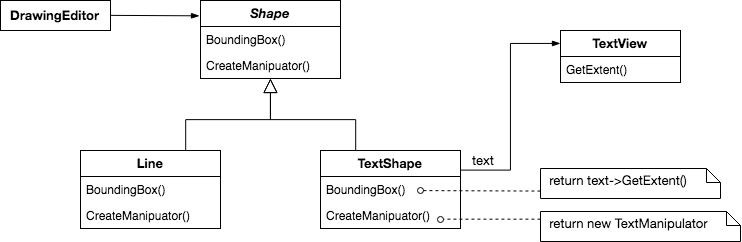
\includegraphics[scale=0.5]{diagrams/adapter_motivation.png}
\end{figure}

This diagram illustrates the object adapter case. It shows how BoundingBox requests, declared in class Shape, are converted to GetExtent requests defined in TextView. Since TextShape adapts TextView to the Shape interface, the drawing editor can reuse the otherwise incompatible TextView class.
\\\\
Often the adapter is responsible for functionality the adapted class doesn't provide. The diagram shows how an adapter can fulfill such responsibilities. The user should be able to "drag" every Shape object to a new location interactively, but TextView isn't designed to do that. TextShape can add this missing functionality by implementing Shape's CreateManipulator operation, which returns an instance of the appropriate Manipulator subclass.
\\\\
Manipulator is an abstract class for objects that know how to animate a Shape in response to user input, like dragging the shape to a new location. There are subclasses of Manipulator for different shapes; TextManipulator, for example, is the corresponding subclass for TextShape. By returning a TextManipulator instance, TextShape adds the functionality that TextView lacks but Shape requires.

\subsection*{Applicability}

Use the Adapter pattern when
\begin{itemize}
    \item you want to use an existing class, and its interface does not match the one you need.
    \item you want to create a reusable class that cooperates with unrelated or unforeseen classes, that is, classes that don't necessarily have compatible interfaces.
    \item (object adapter only) you need to use several existing subclasses, but it's impractical to adapt their interface by subclassing
\end{itemize}

\subsection*{Structure}

A class adapter uses multiple inheritance to adapt one interface to another:

\begin{figure}[H]
\centering
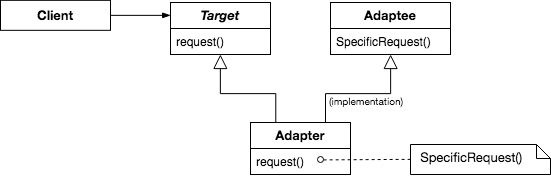
\includegraphics[scale=0.7]{diagrams/adapter_structure_a.png}
\end{figure}

An object adapter relies on object composition:

\begin{figure}[H]
\centering
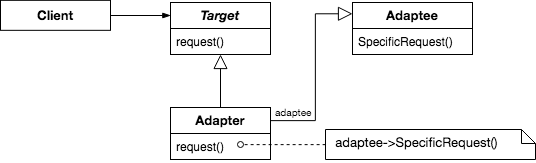
\includegraphics[scale=0.7]{diagrams/adapter_structure_b.png}
\end{figure}

\subsection*{Participants}

\begin{itemize}
    \item Target (Shape)
    \begin{itemize}
        \item defines the domain-specific interface that Client uses.
    \end{itemize}
    \item Client (DrawingEditor)
    \begin{itemize}
        \item collaborates with objects conforming to the Target interface.
    \end{itemize}
    \item Adaptee (TextView)
    \begin{itemize}
        \item defines an existing interface that needs adapting.
    \end{itemize}
    \item Adapter (TextShape)
    \begin{itemize}
        \item adapts the interface of Adaptee to the Target interface.
    \end{itemize}
\end{itemize}

\subsection*{Collaborations}

\begin{itemize}
    \item Clients call operations on an Adapter instance. In turn, the adapter calls Adaptee operations that carry out the request.
\end{itemize}

\subsection*{Consequences}

Class and object adapters have different trade-offs. A class adapter
\begin{itemize}
    \item adapts Adaptee to Target by committing to a concrete Adapter class. As a consequence, a class adapter won't work when we want to adapt a class and all its subclasses.
    \item lets Adapter override some of Adaptee's behavior, since Adapter is a subclass of Adaptee.
    \item introduces only one object, and no additional pointer indirection is needed to get to the adaptee.
\end{itemize}

An object adapter
\begin{itemize}
    \item lets a single Adapter work with many Adaptees—that is, the Adaptee itself and all of its subclasses (if any). The Adapter can also add functionality to all Adaptees at once.
    \item makes it harder to override Adaptee behavior. It will require subclassing Adaptee and making Adapter refer to the subclass rather than the Adaptee itself.
\end{itemize}

Here are other issues to consider when using the Adapter pattern:
\begin{enumerate}

    \item How much adapting does Adapter do? Adapters vary in the amount of work they do to adapt Adaptee to the Target interface. There is a spectrum of possible work, from simple interface conversion—for example, changing the names of operations—to supporting an entirely different set of operations. The amount of work Adapter does depends on how similar the Target interface is to Adaptee's.

    \item Pluggable adapters. A class is more reusable when you minimize the assumptions other classes must make to use it. By building interface adaptation into a class, you eliminate the assumption that other classes see the same interface. Put another way, interface adaptation lets us incorporate our class into existing systems that might expect different interfaces to the class. ObjectWorks/Smalltalk [Par90] uses the term pluggable adapter to describe classes with built-in interface adaptation.
    \\\\
    Consider a TreeDisplay widget that can display tree structures graphically. If this were a special-purpose widget for use in just one application, then we might require the objects that it displays to have a specific interface; that is, all must descend from a Tree abstract class. But if we wanted to make TreeDisplay more reusable (say we wanted to make it part of a toolkit of useful widgets), then that requirement would be unreasonable. Applications will define their own classes for tree structures. They shouldn't be forced to use our Tree abstract class. Different tree structures will have different interfaces.
    \\\\
    In a directory hierarchy, for example, children might be accessed with a GetSubdirectories operation, whereas in an inheritance hierarchy, the corresponding operation might be called GetSubclasses. A reusable TreeDisplay widget must be able to display both kinds of hierarchies even if they use different interfaces. In other words, the TreeDisplay should have interface adaptation built into it.
    \\\\
    We'll look at different ways to build interface adaptation into classes in the Implementation section.

    \item Using two-way adapters to provide transparency. A potential problem with adapters is that they aren't transparent to all clients. An adapted object no longer conforms to the Adaptee interface, so it can't be used as is wherever an Adaptee object can. Two-way adapters can provide such transparency. Specifically, they're useful when two different clients need to view an object differently.
    \\\
    Consider the two-way adapter that integrates Unidraw, a graphical editor framework [VL90], and QOCA, a constraint-solving toolkit [HHMV92]. Both systems have classes that represent variables explicitly: Unidraw has StateVariable, and QOCA has ConstraintVariable. To make Unidraw work with QOCA, ConstraintVariable must be adapted to StateVariable; to let QOCA propagate solutions to Unidraw, StateVariable must be adapted to ConstraintVariable.
    \begin{figure}[H]
    \centering
    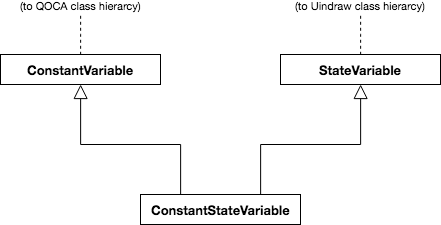
\includegraphics[scale=0.6]{diagrams/adapter_consequence.png}
    \end{figure}
    The solution involves a two-way class adapter ConstraintStateVariable, a subclass of both StateVariable and ConstraintVariable, that adapts the two interfaces to each other. Multiple inheritance is a viable solution in this case because the interfaces of the adapted classes are substantially different. The two-way class adapter conforms to both of the adapted classes and can work in either system.
\end{enumerate}

\section{Composite}

\subsection*{Intent}

Compose objects into tree structures to represent part-whole hierarchies. Composite lets clients treat individual objects and compositions of objects uniformly.

\subsection*{Motivation}

Graphics applications like drawing editors and schematic capture systems let users build complex diagrams out of simple components. The user can group components to form larger components, which in turn can be grouped to form still larger components. A simple implementation could define classes for graphical primitives such as Text and Lines plus other classes that act as containers for these primitives.
\\\\
But there's a problem with this approach: Code that uses these classes must treat primitive and container objects differently, even if most of the time the user treats them identically. Having to distinguish these objects makes the application more complex. The Composite pattern describes how to use recursive composition so that clients don't have to make this distinction.

\begin{figure}[H]
\centering
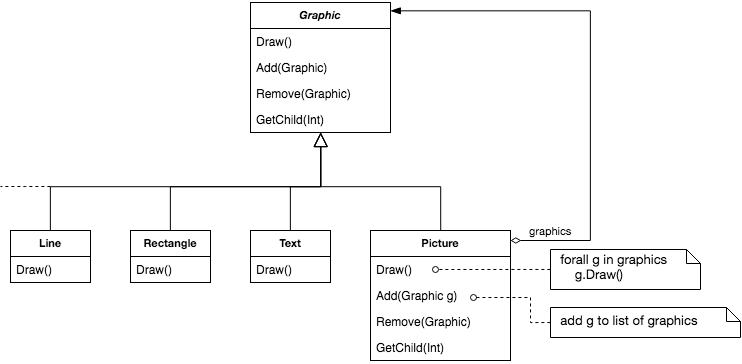
\includegraphics[scale=0.5]{diagrams/composite_motivation.png}
\end{figure}

The key to the Composite pattern is an abstract class that represents both primitives and their containers. For the graphics system, this class is Graphic. Graphic declares operations like Draw that are specific to graphical objects. It also declares operations that all composite objects share, such as operations for accessing and managing its children.
\\\\
The subclasses Line, Rectangle, and Text (see preceding class diagram) define primitive graphical objects. These classes implement Draw to draw lines, rectangles, and text, respectively. Since primitive graphics have no child graphics, none of these subclasses implements child-related operations.
\\\\
The Picture class defines an aggregate of Graphic objects. Picture implements Draw to call Draw on its children, and it implements child-related operations accordingly.
\\\\
Because the Picture interface conforms to the Graphic interface, Picture objects can compose other Pictures recursively.
\\\\
The following diagram shows a typical composite object structure of recursively composed Graphic objects:

\begin{figure}[H]
\centering
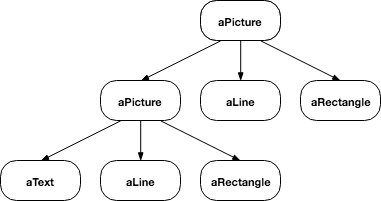
\includegraphics[scale=0.7]{diagrams/composite_motivation_s.png}
\end{figure}

\subsection*{Applicability}

Use the Composite pattern when
\begin{itemize}
    \item you want to represent part-whole hierarchies of objects.
    \item you want clients to be able to ignore the difference between compositions of objects and individual objects. Clients will treat all objects in the composite structure uniformly.
\end{itemize}

\subsection*{Structure}

\begin{figure}[H]
\centering
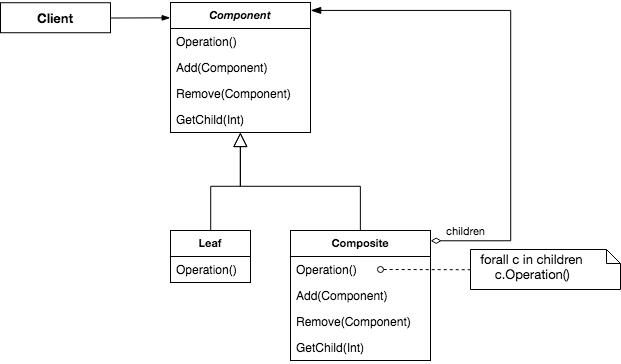
\includegraphics[scale=0.6]{diagrams/composite_structure.png}
\end{figure}

A typical Composite object structure might look like this:

\begin{figure}[H]
\centering
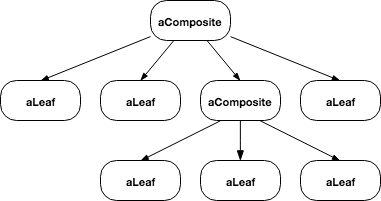
\includegraphics[scale=0.7]{diagrams/composite_structure_s.png}
\end{figure}

\subsection*{Participants}

\begin{itemize}
    \item Component (Graphic)
    \begin{itemize}
        \item declares the interface for objects in the composition.
        \item implements default behavior for the interface common to all classes, as appropriate.
        \item declares an interface for accessing and managing its child components.
        \item (optional) defines an interface for accessing a component's parent in the recursive structure, and implements it if that's appropriate.
    \end{itemize}
    \item Leaf (Rectangle, Line, Text, etc.)
    \begin{itemize}
        \item represents leaf objects in the composition. A leaf has no children.
        \item defines behavior for primitive objects in the composition.
    \end{itemize}
    \item Composite (Picture)
    \begin{itemize}
        \item defines behavior for components having children.
        \item stores child components.
        \item implements child-related operations in the Component interface.
    \end{itemize}
    \item Client
    \begin{itemize}
        \item manipulates objects in the composition through the Component interface.
    \end{itemize}
\end{itemize}

\subsection*{Collaborations}

\begin{itemize}
    \item Clients use the Component class interface to interact with objects in the composite structure. If the recipient is a Leaf, then the request is handled directly. If the recipient is a Composite, then it usually forwards requests to its child components, possibly performing additional operations before and/or after forwarding.
\end{itemize}

\subsection*{Consequences}

The Composite pattern
\begin{itemize}
    \item defines class hierarchies consisting of primitive objects and composite objects. Primitive objects can be composed into more complex objects, which in turn can be composed, and so on recursively. Wherever client code expects a primitive object, it can also take a composite object.
    \item makes the client simple. Clients can treat composite structures and individual objects uniformly. Clients normally don't know (and shouldn't care) whether they're dealing with a leaf or a composite component. This simplifies client code, because it avoids having to write tag-and-case-statement-style functions over the classes that define the composition.
    \item makes it easier to add new kinds of components. Newly defined Composite or Leaf subclasses work automatically with existing structures and client code. Clients don't have to be changed for new Component classes.
    \item can make your design overly general. The disadvantage of making it easy to add new components is that it makes it harder to restrict the components of a composite. Sometimes you want a composite to have only certain components. With Composite, you can't rely on the type system to enforce those constraints for you. You'll have to use run-time checks instead.
\end{itemize}

